\documentclass[12pt]{article}
\usepackage[spanish]{babel}
\usepackage{natbib}
\usepackage{url}
\usepackage[utf8x]{inputenc}
\usepackage{amsmath}
\usepackage{graphicx}
\usepackage{parskip}
\usepackage{fancyhdr}
\usepackage{vmargin}
\usepackage[ddmmyy]{datetime}
\usepackage{anyfontsize}
\usepackage{xcolor}
\setmarginsrb{3 cm}{2.5 cm}{3 cm}{2.5 cm}{1 cm}{1.5 cm}{1 cm}{1.5 cm}

%%%%%%%%%%%%%%%%%%%%%%%%%%%%%%%%%%%%%%%%%%%%%%%%%%%%%%%%%%%%%%%%%%%%%%%%%%%%%%%%%%%%%%%%%
% DATOS GENERALES

\title{Ley de Ohm}	            % Titulo del trabajo.
\author{Nombre Apellido}		% Nombre y apellido
\newcommand{\padron}{105509}    % Padrón
\newcommand{\tpnumber}{1}       % Número de trabajo práctico
\date{\today}					% Fecha (automática, no tocar)

\makeatletter
\let\thetitle\@title
\let\theauthor\@author
\let\thedate\@date
\makeatother

\pagestyle{fancy}
\fancyhf{}
\rhead{\theauthor}
\lhead{\thetitle}
\cfoot{\thepage}

%%%%%%%%%%%%%%%%%%%%%%%%%%%%%%%%%%%%%%%%%%%%%%%%%%%%%%%%%%%%%%%%%%%%%%%%%%%%%%%%%%%%%%%%%
\begin{document}

%% CARATULA - NO TOCAR
\begin{titlepage}
    
\includegraphics[scale = 0.75]{img/logofiuba.png}\\[1.0 cm]	    % Logo fiuba
    \centering
	\textsc{\Large 86.02}\\[0.2 cm]
	\textsc{\large Introducción a la Ingeniería Electrónica}\\[4 cm]
	\textcolor{cyan}{{\fontsize{40}{60}\selectfont \bfseries \thetitle}}\\[0.5cm]
	{ \Large \bfseries Trabajo Práctico N$^\circ$\tpnumber}\\[5cm]
	
	
    \noindent\makebox[\linewidth]{\rule{\textwidth}{0.4pt}}\\[0.5cm]
    \begin{minipage}{.4\textwidth}
    \textbf{Autor}:\\
    \theauthor
    \end{minipage}%
    \begin{minipage}{.4\textwidth}
    \textbf{Padrón}:\\
    \padron
    \end{minipage}%
    \begin{minipage}{.2\textwidth}
    \textbf{Fecha}:\\
    \thedate
    \end{minipage}
 
	\vfill
	
\end{titlepage}

%%%%%%%%%%%%%%%%%%%%%%%%%%%%%%%%%%%%%%%%%%%%%%%%%%%%%%%%%%%%%%%%%%%%%%%%%%%%%%%%%%%%%%%%%

%\tableofcontents    % Comentar o descomentar segun se desee o no una pagina con el indice
%\pagebreak

%%%%%%%%%%%%%%%%%%%%%%%%%%%%%%%%%%%%%%%%%%%%%%%%%%%%%%%%%%%%%%%%%%%%%%%%%%%%%%%%%%%%%%%%%

\section{Sección}

\subsection{Subsección 1}
Inserción de una figura, que se referencia como Fig. \ref{fig:choripan}. La figura se acomoda sola en el lugar más conveniente, y preferentemente al principio de la página. % \ref hace referencia a algo, y entre llaves {} se pone la etiqueta de lo que se quiere referenciar. Al compilar "\ref{...}" se reemplaza por el número de figura o tabla que corresponda.

\begin{figure}
    \centering  %figura centrada en el texto
    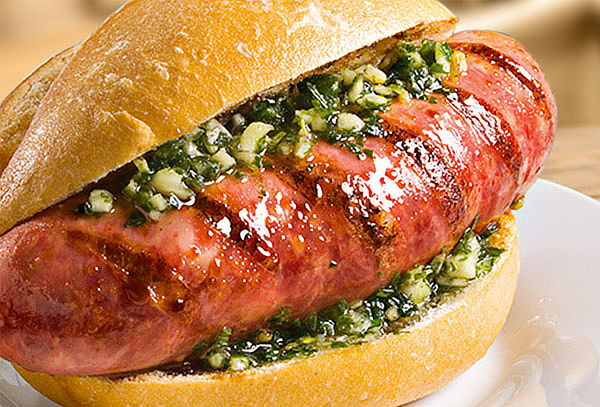
\includegraphics[width=0.4\linewidth]{img/choripan.jpg}  %[width=0.5\linewidth] ancho de la imagen respecto al ancho del texto --- {img/voz_humana.png} path completo de la imagen, en este caso, dentro de la carpeta "img"
    \caption{Un espectacular choripán.}    %texto que acompaña a la imagen por debajo
    \label{fig:choripan}  %etiqueta para referenciar la figura
\end{figure}

\subsection{Subsección 2}
Para cambiar de parrafo, se debe dejar una línea vacía de por medio.

Como sucede aquí.

Si no se deja una línea de por medio,
no se separa en dos párrafos,
como sucede aquí.

\section{Sección 2}

Así se arma una tabla, en este caso la Tabla \ref{tab:temperatura}.

\begin{table}[h!]
  \begin{center}
    \caption{Comentario de la tabla.}
    \label{tab:temperatura}  %etiqueta para referenciar la tabla
    \begin{tabular}{l c|r} % cantidad de columnas que va a tener representadas por las letras l, c, r, que indican el alineamiento (left, center, right). Una barra vertical "|" entre dos letras representa una linea dibujada entre las dos columnas
      Semana & Dia & Temperatura (grados)\\ %los valores de cada columna, se separan con un "&". Al terminar con todas las columnas, se pasa a la siguiente línea con "\\".
      1 & 1 & 25 \\ 
      1 & 2 & 28 \\ 
      1 & 3 & 27 \\ 
      \hline        %este comando entre dos filas, agrega una línea que las separa
      2 & 1 & 26 \\ 
      2 & 2 & 27 \\ 
      \hline
      3 & 1 & 25 \\ 
    \end{tabular}
  \end{center}
\end{table}

\section{Sección 3}

Para insertar símbolos matemáticos en el texto, se encierra la expresión entre signos \$, como se muestra a continuación $\omega$, $\Omega$, $\alpha$, $\beta$. Noten que el símbolo de ohm se representa con la letra griega omega mayúscula $\Omega$. Así es más fácil usar subindices $R_1$ $R_{13}$ y superindices $x^2$ $x^{y+z}$.

Para insertar una ecuación, se puede hacer así

\begin{align}
    V_{12} = I R_1 + I R_2
\end{align}

Para varias ecuaciones:

\begin{align}
    V_{12} = I R_1 + I R_2\\
    V_{12} = 2A \cdot 3\Omega + 2A \cdot 5\Omega\\
    V_{12} = 16V
\end{align}

O asi, donde el símbolo \& se alinea para todas las ecuaciones, sin importar donde esté.

\begin{align}
    V_{12} & = I R_1 + I R_2\\
    V_{12} & = 2A \cdot 3\Omega + 2A \cdot 5\Omega\\
    V_{12} & = 16V
\end{align}

El comando ``cdot'' es conveniente para expresar multiplicación, dejando un espacio entre factores, para mejor entendimiento.

\end{document}
